\section{Iteración IV}
\subsection{Resumen}
En esta iteración se modelaron dos muebles más, tres botones para cambiar de modelo e implementamos un botón para tomar fotografía del escenario.
\subsection{Desarrollo}
Se modelaron dos muebles más, utilizando la misma herramienta, obteniendo los mismos archivos y realizando el proceso de las iteraciones I y II.

En la parte inferior de la aplicación se encuentran tres diseños de muebles, que funcionan como botones para seleccionar el objeto 3D que aparecerá en pantalla.

En la parte superior derecha de la aplicación tenemos ubicado un botón el cual toma una screenshot de la escena y la guarda en el dispositivo.

\begin{figure}[H]
	\centering
	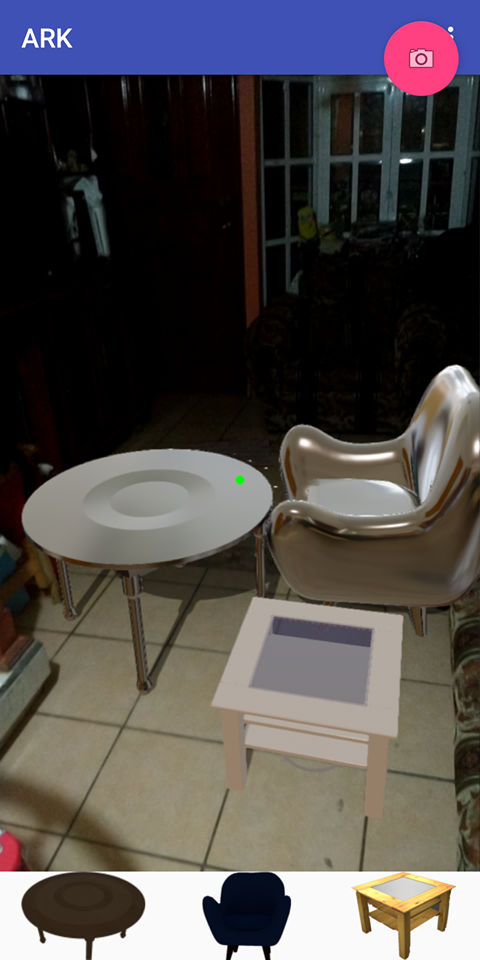
\includegraphics[width=4cm,height=8cm]{imagenes/iteraciones/all.png}
	\caption{Aplicación: modelos en la parte inferior y botón de tomar foto parte superior}
	\label{fig:aplicacion}
\end{figure} 

Al presionar el botón "tomar fotografía" se guardará una imagen de la escena, en formato JPG y aparecerá un mensaje para abrir la ubicación de la imagen.  

\begin{figure}[H]
	\begin{minipage}{0.48\textwidth}
		\centering
		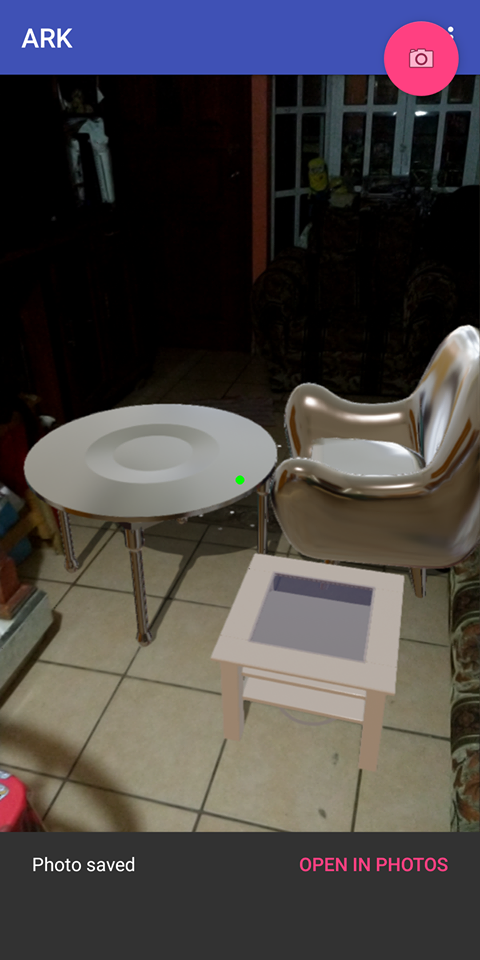
\includegraphics[width=5cm,height=10cm]{imagenes/iteraciones/save1.png}
		\caption{Pantalla de visualización de fotografías}
		\label{fig:save}
	\end{minipage}\hfill
	\begin{minipage}{0.48\textwidth}
		\centering
		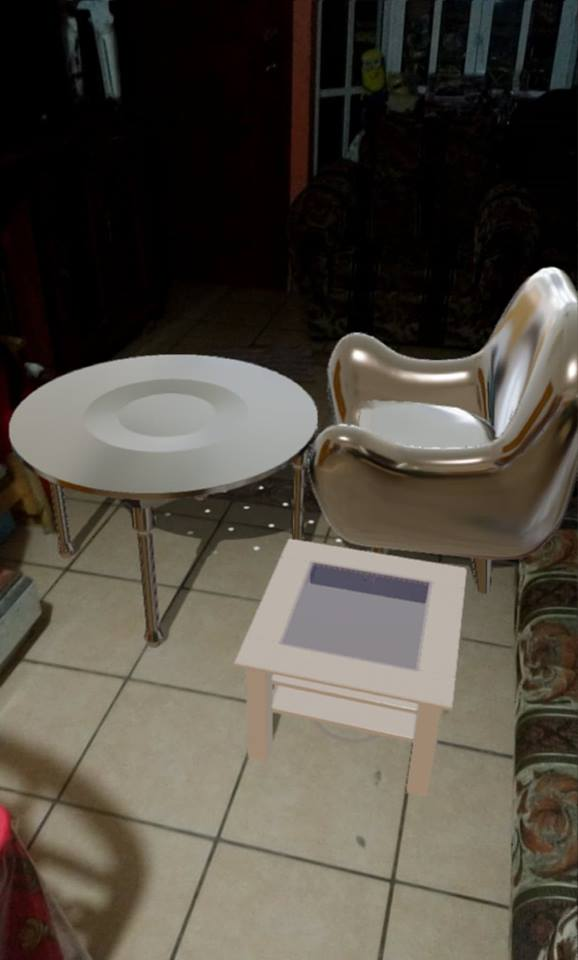
\includegraphics[width=5cm,height=10cm]{imagenes/iteraciones/foto.jpg}
		\caption{Pantalla de registro nuevo usuario}
		\label{fig:foto}
	\end{minipage}\hfill
\end{figure}
Las interfaz que se muestra es temporal, se realizó de esta manera para probar la funcionalidad del aplicación al cumplir con algunos requerimientos funcionales, la interfaz final será como se muestra en los Mockups en la sección de \textbf{Anexos}.

\subsection{Conclusión}
El resultado de ésta iteración será el entregable que mostraremos en la presentación de TT 1. \par
En éste punto nos hemos dado cuenta que la decisión que tomamos de usar ARCore para el desarrollo del proyecto fue correcta. La plataforma funciona de acuerdo a las pruebas de contexto que realizamos al principio y nos ha servido perfectamente para el cumplimiento de algunos requerimientos funcionales planteados en la sección de \textbf{Análisis}. El desarrollo que involucra únicamente la implementación y uso de la realidad aumentada no fue tan problemático. Con respecto a la curva de aprendizaje, estamos por llegar al punto necesario para poder desarrollar el resto de las iteraciones que involucran TT II. \par Al momento de desarrollar las iteraciones, los desarrolladores de Sceneform SDK y ARCore SDK lanzaron nuevas versiones de cada software con correcciones, mejoras, mismas que estaremos probando en las iteraciones posteriores, y seguramente estaremos sustituyendo con las que usamos para las iteraciones ya desarrolladas. 